% !TeX spellcheck = ru_RU_yo
%% -*- coding: utf-8 -*-
\documentclass[12pt,a4paper]{scrartcl} 
\usepackage[T1,T2A]{fontenc}
\usepackage[english,russian]{babel}
\usepackage[utf8]{inputenc}
\usepackage{geometry} 
\geometry{tmargin=2cm,bmargin=2cm,lmargin=3cm,rmargin=1.5cm}
\usepackage{indentfirst}
\usepackage{misccorr}
\usepackage{graphicx}
\usepackage{amsmath}
\usepackage{setspace}
\PassOptionsToPackage{hyphens}{url}
\usepackage[breaklinks]{hyperref}
\usepackage{minted}
\usepackage{textcomp}
\usepackage{comment}
\usepackage{soul}
\usepackage{array}
\usepackage{longtable}
\usepackage{multirow}
\usepackage{makecell}
\usepackage[stable]{footmisc}
\usepackage{listings}
\usepackage{tabularx,booktabs} 
\graphicspath{{images/}}
\usepackage{svg}
\svgpath{{images/}}

%Отключает нумерацию страницы
\pagestyle{empty}

%\titleformat*{\section}{\centering\bfseries}
%\titleformat*{\subsection}{\Large\bfseries}
%\titleformat*{\subsubsection}{\large\bfseries}
%\titleformat*{\paragraph}{\large\bfseries}
%\titleformat*{\subparagraph}{\large\bfseries}

% Команда для линии с нижним подчёркиванием, возможностью написания сверху текста на ней и текстом под ней.
\newcommand\superunderline[3]{$\underset{\text{#3}}{\text{\underline{\hspace{0.3cm}#1\hspace{#2}}}}$}

% Тоже самое, но ещё с отступом слева от текста (выравнивание по середине)
\newcommand\superunderlinec[3]{$\underset{\text{#3}}{\text{\underline{\hspace{#2}#1\hspace{#2}}}}$}

% "Прокаченные" типы колонок для LaTeX. Умеют выравнивать содержимое столбца по горизонтали и принимать фиксированный размер. Полезная вещь.
\newcolumntype{L}[1]{>{\raggedright\let\newline\\\arraybackslash\hspace{0pt}}m{#1}} % Выравнивание по левому краю.
\newcolumntype{C}[1]{>{\centering\let\newline\\\arraybackslash\hspace{0pt}}m{#1}} % Выравнивание по середине.
\newcolumntype{R}[1]{>{\raggedleft\let\newline\\\arraybackslash\hspace{0pt}}m{#1}} % Выравнивание по правому краю.

% Разработка 1993 года: команды, исправляющие неправильные отступы в шапке и подвале колонок в таблицах LaTeX. 
\newcommand\Tstrut{\rule{0pt}{2.6ex}}         % Введи \Tstrut если буквы в таблице налезли на верхнюю полоску
\newcommand\Bstrut{\rule[-0.9ex]{0pt}{0pt}}   % И \Bstrut если буквы "съехали" с середины колонки или наезжают на нижнюю полоску

%Настройки для того, чтобы была возможность переносить строки внутри таблиц. Подробнее здесь:  https://tex.stackexchange.com/questions/2441/how-to-add-a-forced-line-break-inside-a-table-cell
\renewcommand\theadalign{bc}
\renewcommand\theadfont{\normalfont}
\renewcommand\theadgape{\Gape[0pt]}
\renewcommand\cellgape{\Gape[0pt]}

% Убираем варнинг о том что long table представляет собой слишком большой vbox
\makeatletter
\def\LT@start{%
  \let\LT@start\endgraf
  \endgraf\penalty\z@\vskip\LTpre
  \dimen@\pagetotal
  \advance\dimen@ \ht\ifvoid\LT@firsthead\LT@head\else\LT@firsthead\fi
  \advance\dimen@ \dp\ifvoid\LT@firsthead\LT@head\else\LT@firsthead\fi
  \advance\dimen@ \ht\LT@foot
  \edef\restore@vbadness{\vbadness\the\vbadness\relax}% (added)
  \vbadness=\@M % (added)
  \dimen@ii\vfuzz
  \vfuzz\maxdimen
    \setbox\tw@\copy\z@
    \setbox\tw@\vsplit\tw@ to \ht\@arstrutbox
    \setbox\tw@\vbox{\unvbox\tw@}%
  \vfuzz\dimen@ii
  \restore@vbadness % (added)
  \advance\dimen@ \ht
        \ifdim\ht\@arstrutbox>\ht\tw@\@arstrutbox\else\tw@\fi
  \advance\dimen@\dp
        \ifdim\dp\@arstrutbox>\dp\tw@\@arstrutbox\else\tw@\fi
  \advance\dimen@ -\pagegoal
  \ifdim \dimen@>\z@\vfil\break\fi
      \global\@colroom\@colht
  \ifvoid\LT@foot\else
    \advance\vsize-\ht\LT@foot
    \global\advance\@colroom-\ht\LT@foot
    \dimen@\pagegoal\advance\dimen@-\ht\LT@foot\pagegoal\dimen@
    \maxdepth\z@
  \fi
  \ifvoid\LT@firsthead\copy\LT@head\else\box\LT@firsthead\fi\nobreak
  \output{\LT@output}%
}
\makeatother

%Используется для построения подчеркивающих линий
\newlength{\ML}

\setlength{\parskip}{0.5cm}

%\thispagestyle{empty}

\begin{document}
	\phantom{fake text for spacing}
	% ТИТУЛЬНАЯ ЧАСТЬ
	\begin{center}
		\textbf{Министерство науки и высшего образования Российской Федерации} \\
		\textbf{ФГАОУ ВО «Волгоградский государственный университет»} \\
		\textbf{Институт Математики и информационных технологий} \\
		\textbf{Кафедра компьютерных наук и экспериментальной математики} \\
		
		\vspace{0.6cm}
		
		\hfill\begin{minipage}{0.4\textwidth}
		\begin{flushright}
			\textbf{\textsc{УТВЕРЖДАЮ:}} \\
			Зав. кафедрой \textit{КНЭМ} \\
			Клячин В.А.\\
			«\underline{\hspace{0.7cm}}» \underline{\hspace{2.5cm}} 20\underline{\hspace{0.7cm}} г.
		\end{flushright}
		\end{minipage}
		
		\vspace{0.6cm}
		
		\textbf{
			ИНДИВИДУАЛЬНОЕ ЗАДАНИЕ на ПРОИЗВОДСТВЕННУЮ ПРАКТИКУ (ПРЕДДИПЛОМНАЯ)
			\vspace{0.2cm}
		}
		
		\vspace{0.3cm}
		\renewcommand{\arraystretch}{1.5} %!!!
		
		\begin{tabular}{R{3cm}cc}
			Студент & \superunderlinec{\thead{Курбанов Эльдар \\ Ровшанович}}{1.0cm}{(ФИО)} &  \superunderlinec{\thead{МОСм-201}}{1.9cm}{(группа)}
			\vspace{0.6cm} \\
			Руководитель практики от ВолГУ & \superunderlinec{\thead{\phantom{fake text for align}\\Клячин В.А.}}{1.1cm}{(ФИО)} & \superunderlinec{\thead{зав. кафедрой КНЭМ,\\профессор, д.ф.-м.н.}}{0.7cm}{(должность, ученое звание и степень)} \\
			Ответственный за организацию практики от кафедры
 & \superunderlinec{\thead{\phantom{fake text for align}\\Клячин В.А.}}{1.1cm}{(ФИО)} & \superunderlinec{\thead{зав. кафедрой КНЭМ,\\профессор, д.ф.-м.н.}}{0.7cm}{(должность, ученое звание и степень)} \\
			%ragedleft?????? seriously, it works as right align. WTF????
			\multirow{3}{3cm}{\raggedleft Место прохождения практики \phantom{AlignAlign}} & \multicolumn{2}{c}{\underline{\hspace{0.2cm}Лаборатория <<Математического и программного обеспечения\hspace{1cm}}} \\
			& \multicolumn{2}{l}{\superunderlinec{\hspace{0.2cm}ЭВМ>> кафедры КНЭМ ИМИТ ФГАОУ ВолГУ\hspace{3.7cm}}{0cm}{(наименование учреждения, структурного подразделения)}} \\
			Сроки прохождения практики & \multicolumn{2}{l}{с <<29>> апреля 2022 г. \hspace{3cm} по <<16>> мая 2022 г.}
		\end{tabular}
	\end{center}
	%КОНЕЦ ТИТУЛЬНОЙ ЧАСТИ
	
	\newpage
	
	\vspace{0.1cm}
	%1 раздел
	1. Содержание и задания практики:
		%\newpage
		\begin{longtable}{| L{0.7cm} | L{1.9cm}| L{5.3cm} | L{1cm} | L{2.1cm} | L{1.7cm} |}
			\hline % Требуется для рисования горизонтальной линии.
			\centering{№ п/п} &	\centering{Этапы практики} & \centering{Содержание работы и задания этапов} & \Tstrut \centering{Коли-чество часов} & \Tstrut \centering{Календар-ные сроки проведе-ния} & Форма отчётности \\
			\hline
			% Используем Bstrut и Tstrut в необходимых местах чтобы чинить вёрстку таблицы. Как можете заметить, выше пришлось вручную переносить слова при помощи "-". К сожалению, Bstrut и Tstrut ломают автоматические переносы цельных слов в LaTeX.
			1 & \Tstrut Подгото-витель-ный этап \Bstrut & Решение организационных вопросов: установочная конференция, знакомство с задачами и программой практики, требованиями к отчетной документации; знакомство с объектами и особенностями предстоящей деятельности; инструктаж по технике безопасности & 10 & 29.04.2022 & Собеседование \\
			\hline
			2 & Ориентировочный этап & Знакомство с базовой организацией практики, изучение и анализ/обзор нормативно-правовой документации; знакомство с методами работы; изучение/обзор литературы; знакомство с методами исследования. & 18 & 30.04.2022-04.05.2022 & Собеседование. Письменный отчет (часть). \Bstrut \\
			\hline
			3 & Основной этап & Подготовка научно-аналитического обзора по выбранной тематике на основе последних публикаций в российских и зарубежных журналах для анализа существующих решений по заданной предметной области.
Построение функциональной модели или диаграммы классов для описания поставленной задачи (Описание структурных элементов исследования, их связи, возможные форматы представляемых в системе данных. Анализ особенностей решаемой задачи.). Представление методов оценки качества проектного решения (например, результатов тестирования). & 60 & 05.05.2022-12.05.2022 & Письменный отчёт (часть). \\
			\hline
			4 & Заключи-тельный этап & Подготовка отчета о прохождении практики. Выступление с докладом-презентацией. & 20 & 13.05.2022-16.05.2022 & Письменный отчет (оформление). Представление/защита результатов практики. \\
			\hline
		\end{longtable}
	
		2. Планируемые результаты практики:\\
		\textit{студент должен знать}: основы в области математики, программирования и информационных технологий; методы построения научной работы, современные методы сбора и анализа полученного материала, способы аргументации; основы построения научных обзоров, публикаций, рефератов и библиографий по тематике проводимых исследований на русском и английском языках; особенности распоряжения правами на
результаты интеллектуальной деятельности; формы и методы правовой охраны результатов интеллектуальной деятельности; современными технологиями проектирования и производства программного продукта; направления развития: компьютеров с традиционной (нетрадиционной) архитектурой; современных систем программных средств, операционных систем, операционных и сетевых оболочек, сервисных программ; тенденции развития функций и архитектур проблемно-ориентированных программных систем и комплексов в профессиональной деятельности; концептуальные положения функционального, логического, объектно-ориентированного и визуального направлений программирования, методы, способы и средства разработки программ в рамках этих направлений; современные методы разработки и реализации алгоритмов математических моделей на базе языков и пакетов прикладных программ моделирования; основные стандарты, нормы и правила разработки технической документации программных продуктов и программных комплексов.


		\textit{студент должен уметь}: находить, формулировать и решать стандартные задачи в собственной научно-исследовательской деятельности в области программирования и информационных технологий; решать научные задачи в связи с поставленной целью и в соответствии с выбранной методикой; решать задачи, связанные с использованием
результатов интеллектуальной деятельности и средств индивидуализации для создания инновационной продукции и услуг, в том числе ориентированных на зарубежные рынки; использовать технологии проектирования при создании программных продуктов; программировать для компьютеров с различной современной архитектурой; программировать в рамках функционального, логического, объектно-ориентированного и визуального направлений; разрабатывать и реализовывать алгоритмы математических моделей на базе языков и пакетов прикладных программ моделирования; подготовить техническую документацию программных продуктов.


		\textit{студент должен владеть умениями}: научно-исследовательской деятельности в области
программирования и информационных технологий; выступлений и научной
аргументации и профессиональной деятельности; выполнять оценку преимуществ новой
технологии по сравнению с аналогами; применения технологий проектирования при создании программных продуктов; выбора архитектуры и комплексирования современных компьютеров, систем, комплексов и сетей системного администрирования; разработки программ в рамках функционального, логического, объектно-ориентированного и визуального направлений; разработки и реализации алгоритмов их на базе языков и пакетов прикладных программ моделирования; подготовки технической документации.

		\vspace{0.5cm}

		\hfill\begin{minipage}{0.7\textwidth}
			Студент \hspace{0.2cm} \superunderlinec{\phantom{Курбанов Э.Р.}}{0.3cm}{(подпись)} \hspace{1.01cm} \superunderlinec{\phantom{Курбанов Э.Р.}}{0.49cm}{(расшифровка подписи)} \\
			\vspace{0.2cm}
		\end{minipage}
		\hfill\begin{minipage}{\textwidth}
			Руководитель практики от ВолГУ \hspace{0.2cm} \superunderlinec{\phantom{Курбанов Э.Р.}}{0.3cm}{(подпись)} \hspace{1cm} \superunderlinec{Клячин В.А.}{0.6cm}{(расшифровка подписи)} \\
		\end{minipage}
	    \hfill\begin{minipage}{\textwidth}
	     \hspace{0.6cm}Ответственный за организацию\\\phantom{для выравни}практики от кафедры\hspace{0.25cm} \superunderlinec{\phantom{Курбанов Э.Р.}}{0.3cm}{(подпись)} \hspace{1cm} \superunderlinec{Клячин В.А.}{0.6cm}{(расшифровка подписи)} \\
	    \end{minipage}
	
	\newpage
	
	% ТИТУЛЬНАЯ ЧАСТЬ
	\begin{center}
		\textbf{Министерство науки и высшего образования Российской Федерации} \\
		\textbf{ФГАОУ ВО «Волгоградский государственный университет»} \\
		\textbf{Институт математики и информационных технологий} \\
		\textbf{Кафедра компьютерных наук и экспериментальной математики} \\
		
		\vspace{0.6cm}
		
		\hfill\begin{minipage}{0.4\textwidth}
		\begin{flushright}
			\textbf{\textsc{УТВЕРЖДАЮ:}} \\
			Зав. кафедрой \textit{КНЭМ} \\
			Клячин В.А.\\
			«\underline{\hspace{0.7cm}}» \underline{\hspace{2.5cm}} 20\underline{\hspace{0.7cm}} г.
		\end{flushright}
		\end{minipage}
		
		\vspace{0.6cm}
		
		\textbf{
			ОТЧЕТ\\О ПРОХОЖДЕНИИ ПРОИЗВОДСТВЕННОЙ ПРАКТИКИ\\(ПРЕДДИПЛОМНАЯ)
			\vspace{0.2cm}
		}
		
		\vspace{0.3cm}
		\renewcommand{\arraystretch}{1.5} %!!!
		
		\begin{tabular}{R{3cm}cc}
			Студент & \superunderlinec{\thead{\normalfont{Курбанов Эльдар} \\ \normalfont{Ровшанович}}}{1.0cm}{(ФИО)} &  \superunderlinec{\thead{\normalfont{МОСм-201}}}{1.9cm}{(группа)}
			\vspace{0.6cm} \\
			Руководитель практики от ВолГУ & \superunderlinec{\thead{\normalfont{\phantom{fake text for align}}\\\normalfont{Клячин В.А.}}}{1.1cm}{(ФИО)} & \superunderlinec{\thead{\normalfont{зав. кафедрой КНЭМ,}\\\normalfont{профессор., д.ф.-м.н.}}}{0.7cm}{(должность, ученое звание и степень)} \\
			Ответственный за организацию практики от кафедры
			& \superunderlinec{\thead{\normalfont{\phantom{fake text for align}}\\\normalfont{Клячин В.А.}}}{1.1cm}{(ФИО)} & \superunderlinec{\thead{\normalfont{зав. кафедрой КНЭМ,}\\\normalfont{профессор., д.ф.-м.н.}}}{0.7cm}{(должность, ученое звание и степень)} \\
			%ragedleft?????? seriously, it works as right align. WTF????
			\multirow{3}{3cm}{\raggedleft Место прохождения практики \phantom{AlignAlign}} & \multicolumn{2}{c}{\underline{\hspace{0.2cm}Лаборатория <<Математического и программного обеспечения\hspace{1cm}}} \\
			& \multicolumn{2}{l}{\superunderlinec{\hspace{0.2cm}ЭВМ>> кафедры КНЭМ ИМИТ ФГАОУ ВолГУ\hspace{3.7cm}}{0cm}{(наименование учреждения, структурного подразделения)}} \\
			
			Сроки прохождения практики & \multicolumn{2}{c}{с <<29>> апреля 2022 г. \hspace{2cm} по <<16>> мая 2022 г.}
		\end{tabular}
	\end{center}
	%КОНЕЦ ТИТУЛЬНОЙ ЧАСТИ
	
	\newpage
	
	\begin{center}
		\textbf{1. Ход выполнения практики}
	\end{center}

\renewcommand\theadalign{bl}

	\begin{longtable}{| C{0.6cm} | C{2cm}| C{2cm} | L{5.5cm} | C{2.58cm} |}
		\hline % Требуется для рисования горизонтальной линии.
		№ п/п &	Этап практики & Дата & \centering Описание выполненной работы & \Tstrut Отметки руководителя о выполнении \\
		\hline
		% Используем Bstrut и Tstrut в необходимых местах чтобы чинить вёрстку таблицы. Как можете заметить, выше пришлось вручную переносить слова при помощи "-". К сожалению, Bstrut и Tstrut ломают автоматические переносы цельных слов в LaTeX.
		1 & Подготовительный этап & 29.04.2022 \Bstrut & Решение организационных вопросов: установочная конференция, знакомство с задачами и программой практики, требованиями к отчетной документации; знакомство с объектами и особенностями предстоящей деятельности; инструктаж по технике безопасности & \\
		\hline
		2 & Ориентировочный этап & 30.04.2022-04.05.2022 \Bstrut & Знакомство с базовой организацией практики, изучение и анализ/обзор нормативно-правовой документации; знакомство с методами работы; изучение/обзор литературы; знакомство с методами исследования. & \\
		\hline
		\multirow{10}{0.6cm}{\centering 3} & \multirow{10}{2cm}{\centering Основной этап} & 05.05.2022 \Bstrut & \Tstrut Подготовка научно-аналитического обзора по выбранной тематике на основе последних публикаций в российских и зарубежных журналах для анализа существующих решений по заданной предметной области. & \\
		\cline{3-5}
		& & 06.05.2022-11.05.2022 \Bstrut & \Tstrut Построение функциональной модели или диаграммы классов для описания поставленной задачи (Описание структурных элементов исследования, их связи, возможные форматы представляемых в системе данных. Анализ особенностей решаемой задачи.). & \\
		\cline{3-5}
		& & 12.05.2022 \Bstrut & \Tstrut Представление методов оценки качества проектного решения (например, результатов тестирования). & \\
		\hline
		4 & Заключительный этап & 13.05.2022-16.05.2022 \Bstrut & \Tstrut Подготовка отчета о прохождении практики. Выступление с докладом-презентацией. & \\
		\hline
		
	\end{longtable}

\renewcommand\theadalign{bc}
	
	\vspace{0.5cm}
	\hfill\begin{minipage}{0.7\textwidth}
		Студент \hspace{0.2cm} \superunderlinec{\phantom{Курбанов Э.Р.}}{0.3cm}{(подпись)} \hspace{1cm} \superunderlinec{Курбанов Э.Р.}{0.3cm}{(расшифровка подписи)} \\
	\end{minipage}
	
	%КОНЕЦ ПЕРВОЙ СЕКЦИИ
	
	\newpage
		
		\begin{center}
			\textbf{ОТЗЫВ РУКОВОДИТЕЛЯ ОТ УНИВЕРСИТЕТА} \\
			\vspace{0.5cm}
			\noindent
			\underline{\hspace{15cm}} \\
			\vspace{0.3cm}\underline{\hspace{15cm}} \\
			\vspace{0.3cm}\underline{\hspace{15cm}} \\
			\vspace{0.3cm}\underline{\hspace{15cm}} \\
			\vspace{0.3cm}\underline{\hspace{15cm}} \\
			\vspace{0.3cm}\underline{\hspace{15cm}} \\
			\vspace{0.3cm}\underline{\hspace{15cm}} \\
			\vspace{0.3cm}\underline{\hspace{15cm}} \\
			\vspace{0.3cm}\underline{\hspace{15cm}} \\
			\vspace{0.3cm}\underline{\hspace{15cm}} \\
			\vspace{0.3cm}\underline{\hspace{15cm}} \\
			\vspace{0.3cm}\underline{\hspace{15cm}} \\
			\vspace{0.3cm}\underline{\hspace{15cm}} \\
			\vspace{0.3cm}\underline{\hspace{15cm}} \\
			\vspace{0.3cm}\underline{\hspace{15cm}} \\
			\vspace{0.3cm}\underline{\hspace{15cm}} \\
			\vspace{0.3cm}\underline{\hspace{15cm}} \\
			\vspace{0.3cm}\underline{\hspace{15cm}} \\
		\end{center}
		
		\renewcommand{\arraystretch}{2} %!!!
		\renewcommand\theadalign{br}
		
		\begin{tabular}{R{5cm}cc}
			Зачёт по практике принят с оценкой & \superunderlinec{}{2.22cm}{(по 5-балльной шкале)} &  \superunderlinec{}{2.22cm}{(по 100-бальной шкале)} \\
			Ответственный за организацию практики от \phantom{sdfsdfsdfsdsdf} кафедры «\underline{\hspace{0.7cm}}» \underline{\hspace{2.1cm}} 20\underline{\hspace{0.6cm}} г. & \superunderlinec{}{2.22cm}{(подпись)} & \Tstrut\superunderlinec{Клячин В.А.}{1cm}{(расшифровка подписи)} \\
			Руководитель практики \phantom{sdfsdfsdfsdsdf} от ВолГУ «\underline{\hspace{0.7cm}}» \underline{\hspace{2.1cm}} 20\underline{\hspace{0.6cm}} г. & \superunderlinec{}{2.22cm}{(подпись)} & \Tstrut\superunderlinec{Клячин В.А.}{1cm}{(расшифровка подписи)} \\
		\end{tabular}
		
		\newpage
	
	\begin{center}
		\textbf{Приложения\footnote{Приложения к отчету о прохождении практики: (приводится материалы, указанные в индивидуальном плане на практику в графе «Форма отчетности», например, научно-исследовательская работа, презентации, конспект занятия и т.д.).}}
	\end{center}
		
		\section*{Вступление}
			В ходе практики я работал над корректным подсчётом пройденного роботом расстоянием. Это позволит роботу самому оценивать его текущее местоположение на карте, выстраиваемой при помощи лазерного сканера LiDAR. Сам робот представляет собой платформу на двух гусеницах и оснащён двумя электродвигателями, драйвером, лазерным сканером и компьютером, управляющий процессом движения. Он изображён на Рисунке \ref{fig:Robot}.
			
			\begin{figure}[h]
				\center{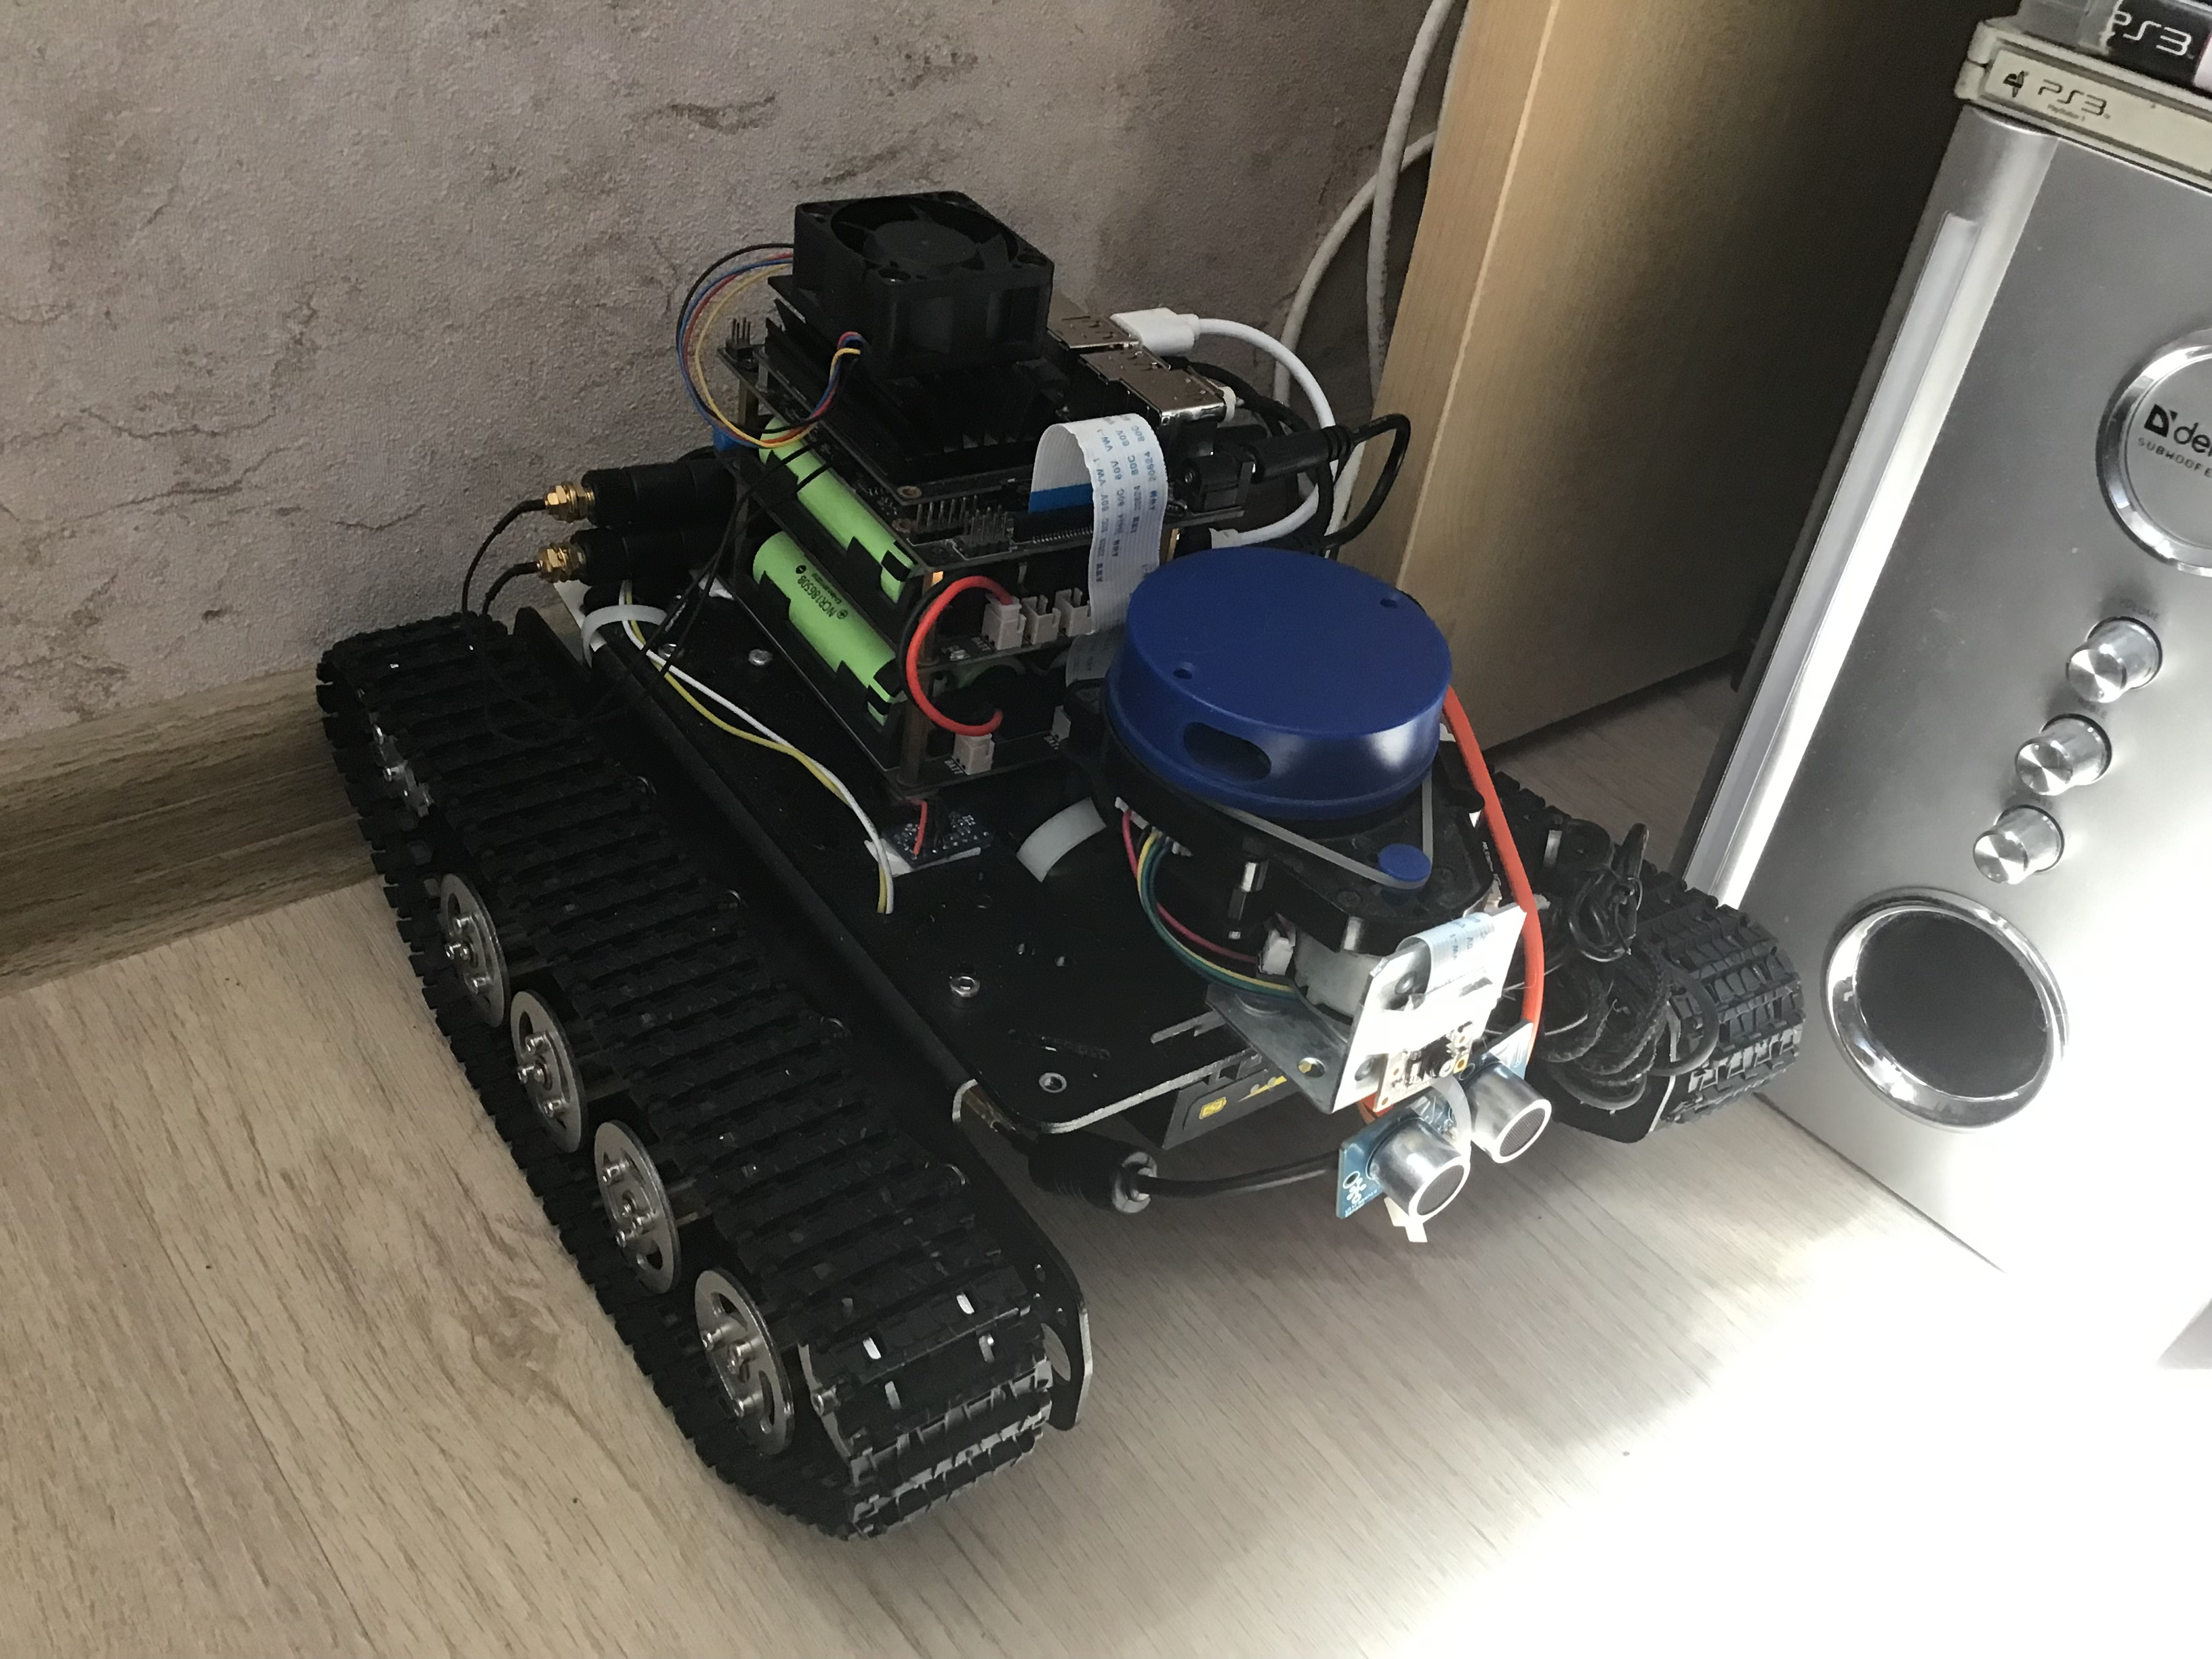
\includegraphics[width=0.6\linewidth]{robot.jpeg}}
				\caption{Робот}
				\label{fig:Robot}
			\end{figure}
			
			Моей задачей стало исправление некорректного подсчёта числа оборотов колеса производимых на ведущей части гусеницы робота. Для успешного построения карты местности (пример изображён на Рисунке \ref{fig:Map}) при помощи лазерного сканера, изображённого на Рисунке \ref{fig:X4} роботу необходимо решать задачу локализации в пространстве. Погрешностей в определении местоположения должно быть как можно меньше, они напрямую будут влиять на выстраиваемую карту местности. Будут возникать смещения или ещё хуже - артефакты\footnote{объекты на карте, которых в реальности не существует}.
			
			\begin{figure}[h]
				\center{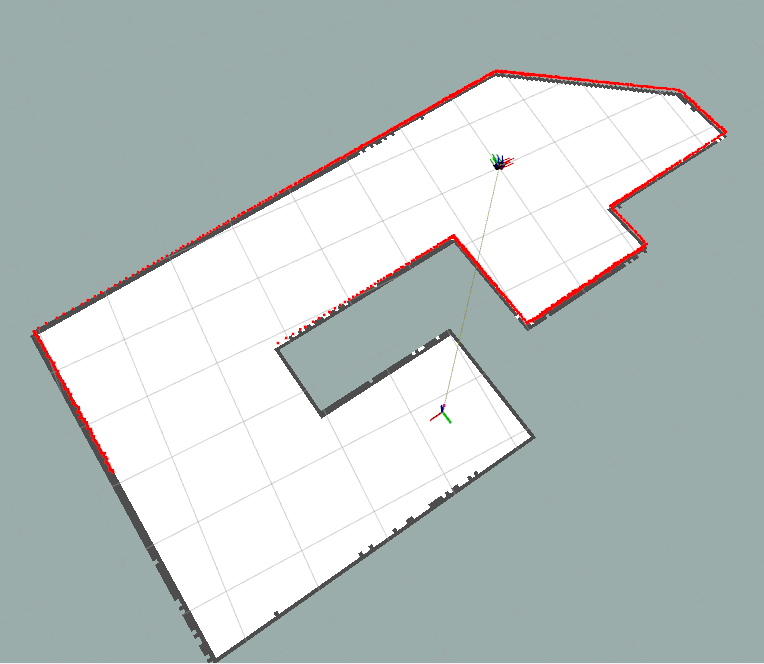
\includegraphics[width=0.6\linewidth]{rviz_map.png}}
				\caption{Карта местности, построенная при помощи лазерного сканирования}
				\label{fig:Map}
			\end{figure}
			
			\begin{figure}[h]
				\center{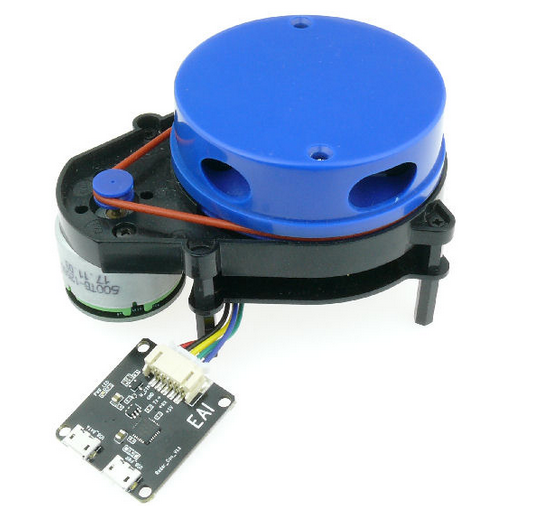
\includegraphics[width=0.6\linewidth]{ydlidar_x4.png}}
				\caption{Лазерный сканер YDLIDAR X4}
				\label{fig:X4}
			\end{figure}
			
			На данном роботе возможно реализовать три способа локализации в пространстве:
			\begin{enumerate}
				\item Анализ смещения облака точек;
				\item Подсчёт одометрии;
				\item Первые два способа вместе, корректирующие показатели друг друга.
			\end{enumerate}
			
			Такие способы локализации, как триангуляция на основе заранее установленных радиомаяков и спутниковая связь Глонасс не рассматриваются ввиду требования полной автономности робота.
			
		\section*{Практика}
			Моей задачей является - "исправление расчета оборотов ведущего колеса гусеничного шасси робота". На основе этих оборотов считается фактически пройденное роботом расстояние после применения команды движения в определённую сторону. Обнаружилось, что получаемые значения оборотов отличались от ожидаемых при высокой загруженности управляющего компьютера. Изначально исправлению подлежала только программная часть робота, однако в ходе работы выяснилось, что природа ошибки кроется в операционной системе робота. 
			
			Принцип получения показателей пройденного роботом расстояния следующий:
			\begin{itemize}
				\item Робот включается и инициализирует среду ROS\footnote{Robot Operating System};
				\item Включается система навигации робота, которая требует лазерный сканер и текущее расстояние, пройденное гусеницами;
				\item Запускается лазерный сканер и происходит инициализация аппаратного интерфейса GPIO с цифровыми электрическими входами;
				\item Навигационная система по шине I$^2$C даёт команду драйверам двигателя на движение;
				\item Датчики Холла, установленные на двигателях робота подают электрический сигнал 3.3 вольт в момент прохождения колесом одного оборота.
				\item Аппаратный интерфейс GPIO считывает данный сигнал и суммирует все такие обороты;
				\item На основе новых пройденных роботов подсчитывается пройденное роботом расстояние.
			\end{itemize}
			
		\section*{1 этап}
			Первоначально я посчитал, что причиной расхождения показателей является подвисание программы на каком-либо из циклов в программном коде и при высокой загруженности мы просто не успеваем исполнить код, отвечающей за чтение цифрового сигнала на интерфейсе GPIO. В таком случае вполне возможно мы могли недосчитаться каких-то оборотов колеса и избавление от таких циклов станет решением проблемы.
			
			Т.к. речь идёт о программном коде робота и мы имеем дело с Robot Operating System, оперирующей с входными данными, как с входящими в неё топиками, которые публикуют другие узлы, я нашёл какой узел отвечает за публикацию и суммирование текущих оборотов двигателя. Искать долго не пришлось, но никаких бесконечных циклов в коде узла и библиотеки Jetson.GPIO, которую он использует найдено не было. Каких-либо мест в коде, где исполнение узла могло бы застревать найдено не было. 
			
			Мною была выдвинута идея о том, что такие просчёты со стороны узла напрямую связаны с природой операционной системы Ubuntu, используемой на роботе. Данная ОС не является системой, нацеленной на исполнение команд в режиме реального времени, а это значит, что в момент прохождения ведущим колесом робота датчика Холла мы не можем гарантировать квант времени от операционной системы на исполнение программы нашего узла, а значит не можем и гарантировать подсчёт всех оборотов колеса. Примерная схема такого просчёта представлена на Рисунке \ref{fig:Miscount}
			
			\begin{figure}[h]
				\center{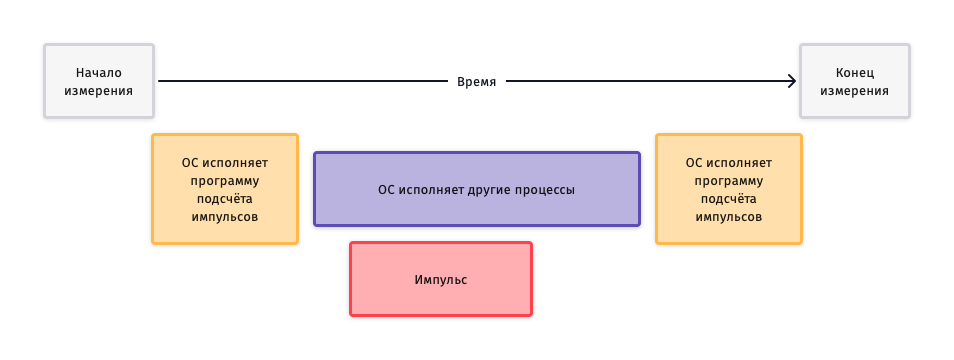
\includegraphics[width=\linewidth]{Miscount.png}}
				\caption{Пример импульса, который не будет подсчитан программой}
				\label{fig:Miscount}
			\end{figure}
			
			Заручившись поддержкой тематических интернет-форумов и своего научного руководителя, я приступил ко второму этапу...
			
		\section*{2 этап}
			Выходом из данной ситуации стало бы использование операционной системы реального времени, такой как QNX\footnote{QNX (произносится «кьюникс», «кью-эн-экс») — POSIX-совместимая операционная система реального времени, предназначенная преимущественно для встраиваемых систем. Считается одной из лучших реализаций концепции микроядерных операционных систем.}, но это стало не позволительной роскошью для данного робота в следствии отсутствия какой-либо рабочей реализации используемого фреймворка ROS для данной ОС, а также высокая стоимость лицензии.
			
			По названным выше причинам было решено некоторый микроконтроллер, который удовлетворял следующим требованиям:
			\begin{enumerate}
				\item Принимает электрические сигналы в реальном времени без просчётов
				\item Способна коммуницировать с Robot Operating System
				\item Является компактным и энергоэффективным решением
			\end{enumerate}
			
			Под эти требования отлично подошёл микроконтроллер Teensy 4.0 на базе 32 битного ARM процессора NXP MIMXRT1062DVL6A. Схематичное описание и внешний вид микрокомпьютера представлены на Рисунке 
			
			\begin{figure}[h]
				\center{
					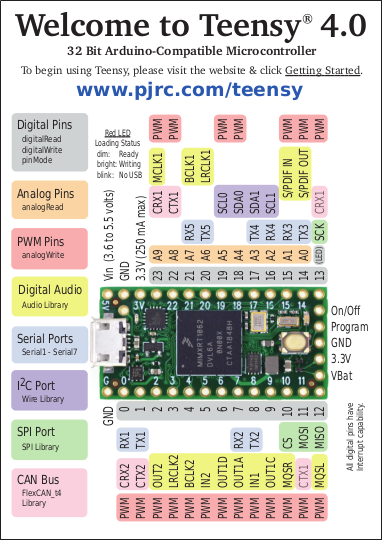
\includegraphics[width=0.45\linewidth]{teensy40_card10a_rev2.png}
					\hspace{0.5cm}
					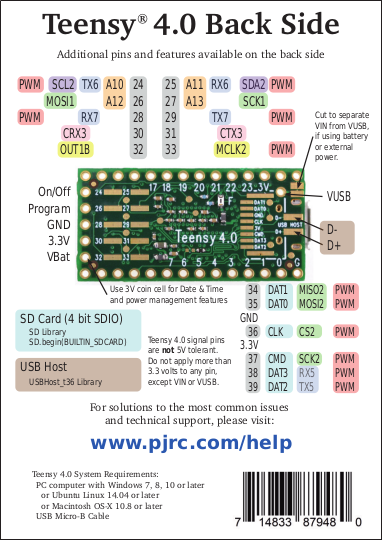
\includegraphics[width=0.45\linewidth]{teensy40_card10b_rev2.png}
				}
				\caption{Описание микрокомпьютера Teensy 4.0}
				\label{fig:TeensyDesc}
			\end{figure}
			
			К нему были подсоединены датчики холла и внешние электропитание 5 вольт. В последствии планируется делегировать на данный микроконтроллер нагрузку, связанную с управлением драйвером электродвигателей робота.
			
			После проверки цепей питания и удостоверившись в корректном прохождении сигналов к микроконтроллеру, я начал реализовывать программную часть.
			
		\section*{3 этап}
			Для реализации программной части необходимо использовать систему разработки Arduino IDE с установленным дополнением TeensyDuino. Это позволяет использовать все библиотеки, доступные для Arduino доступными и для микроконтроллера Teensy 4.0. 
			
			Для коммуникации между основным компьютером NVIDIA Jetson Xavier NX и Teensy 4.0 было решено использовать предоставляемый фреймворком ROS инструмент rosserial. Данный инструмент позволяет при помощи Arduino-совместимой библиотеки и подключения по серийному порту наладить полноценную в рамках ROS коммуникацию в режиме реального времени без необходимости вручную описывать взаимодействие между двумя компьютерами.
			
			Идея взаимодействия будет следующая:
			\begin{enumerate}
				\item На основном компьютере запускается ROS, который при помощи rosserial устанавливает соединение с Teensy
				\item Микроконтроллер считает количество пришедших электрических сигналов
				\item Каждый ROS цикл публикуется количество подсчитанных сигналов
				\item Узел на стороне главного компьютера принимает и обрабатывает данные числа для подсчёта местоположения робота
			\end{enumerate}
			
			Реализация скетча представлена в Листинге ...
			
			\begin{lstlisting}[language=C,caption={Формат сообщения nav\_msgs/Odometry},label={lst:OdometryMsg}]
std_msgs/Header header
string child_frame_id
geometry_msgs/PoseWithCovariance pose
geometry_msgs/TwistWithCovariance twist
			\end{lstlisting}	
			
			После завершения работы мои проверки не показали расхождений в значении подсчитанных оборотов ведущих колёс робота и я посчитал данную задачу завершённой.
			
		\end{document}